% Qualitative figure. Requires \ptag (defined in both manuscript preambles) and graphicx.
% Source PDF: reports/paper_figure/scene_open_drawer.pdf
%   scripts/modality_demo.py  --ckpt outputs/arm6__seed42_fi3_512_aug_sr/checkpoint-9000/step9000.ckpt
%   scripts/paper_figure_modalities.py --no-gt --per-scene --cell 132 --frames 0,8,16,24,32,40
\begin{figure}[t]
\centering
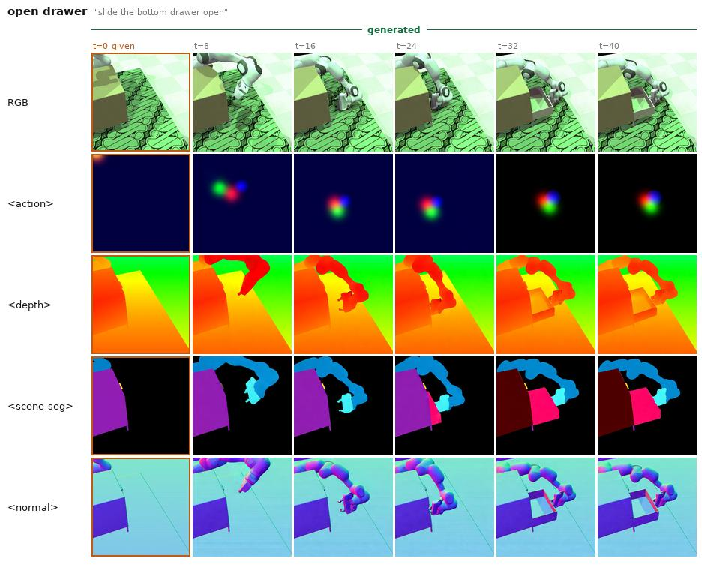
\includegraphics[width=\linewidth]{figures/scene_open_drawer.pdf}
\caption{\textbf{One checkpoint, four prompts.} Every row is produced by the same arm6 model
(step 9{,}000) from the same episode, window, views and seed; the only thing that differs between
rows is the prompt prefix --- \ptag{video}\ptag{action}, \ptag{video}\ptag{depth},
\ptag{video}\ptag{scene-seg}, \ptag{video}\ptag{normal}. Columns are frames $0,8,16,24,32,40$ of a
$41$-frame window spanning $6.0$\,s, so each row is a filmstrip: the model emits a \emph{video} in
every modality, from one shared output head and one loss. Conditioning is \texttt{IIII}, the regime
a closed-loop rollout uses: only the first latent frame of each segment is given (orange,
\texttt{t=0}) and everything to its right is generated. Pixels are the model's raw canvas, not a
decoded re-rendering --- depth is the RGB-cube path image and segmentation the nine-role palette.
View~0 of~2; instruction \emph{``slide the bottom drawer open''}. Decoded against ground truth this
sample gives AbsRel $0.088$ for depth, macro-mIoU $0.435$ for the role map, and mean cosine
$0.895$ for normals.}
\label{fig:qualitative}
\end{figure}
